\section{Лабораторная работа \textnumero{}2: ParaView}

\subsection{Цель работы}

Освоить запись результатов расчёта в формат VTK и визуализацию
нестационарных процессов в ParaView на примере распространения
ударной волны в трёхмерной неструктурированной сетке.

\subsection{Постановка задачи}

На сетке из предыдущей лабы (карандаш \texttt{pencil.stl}) моделируется
распространение сферической ударной волны от точечного источника.
В каждом узле сетки на каждом временном шаге вычисляются скалярное
поле давления $p$ и векторное поле скоростей $\mathbf{v}$.

\subsection{Физическая модель}

Волна задаётся аналитически как гауссов импульс, распространяющийся
со скоростью $c$ от точки $(x_0, y_0, z_0)$:
\begin{equation}
  p(\mathbf{x}, t) = v_0
    \exp\!\left(-\frac{(r - ct)^2}{\sigma^2}\right)
    \cdot A(r),
  \qquad r = |\mathbf{x} - \mathbf{x}_0|,
\end{equation}
где затухание $A(r)$ моделирует геометрическое и вязкое рассеяние:
\begin{equation}
  A(r) = \frac{e^{-\alpha r}}{1 + \beta r},
  \quad \alpha = 0.005,\quad \beta = 0.02.
\end{equation}

Отражения от торцов по оси $z$ учитываются зеркальными источниками
с коэффициентом отражения $0.8$ (первый порядок) и $0.64$ (второй порядок).

\subsection{Реализация}

\subsubsection{Загрузка сетки}

Сетка загружается из \texttt{.msh}-файла через gmsh API, узлы и
3D-элементы сохраняются во внутренних структурах \texttt{Node} и
\texttt{Cell}.

\begin{lstlisting}[language=C++, caption={Загрузка узлов из .msh}]
gmsh::model::mesh::getNodes(nodeTags, coords, parametricCoords);
for (size_t i = 0; i < nodeTags.size(); ++i) {
    nodes_[i].x = coords[3*i + 0];
    nodes_[i].y = coords[3*i + 1];
    nodes_[i].z = coords[3*i + 2];
    tag_to_index[nodeTags[i]] = i;
}
\end{lstlisting}

\subsubsection{Временной цикл}

На каждом шаге для каждого узла вычисляется вклад прямой волны
и четырёх зеркальных источников:

\begin{lstlisting}[language=C++, caption={Вычисление поля в узле}]
void PointHit(Node &node, double t) {
    applyWave(hit_center_, node, t, c_, v0_, sigma_);

    Node mirror_top(cx, cy, 2.0*z_max_ - hit_center_.z);
    applyWave(mirror_top,  node, t, c_, v0_*0.8, sigma_);

    Node mirror_bot(cx, cy, 2.0*z_min_ - hit_center_.z);
    applyWave(mirror_bot,  node, t, c_, v0_*0.8, sigma_);
}
\end{lstlisting}

\subsubsection{Запись кадров в VTK}

Каждый кадр записывается в отдельный \texttt{.vtu}-файл:

\begin{lstlisting}[language=C++, caption={Запись кадра в VTK}]
auto grid   = vtkSmartPointer<vtkUnstructuredGrid>::New();
auto smth   = vtkSmartPointer<vtkDoubleArray>::New();
auto vel    = vtkSmartPointer<vtkDoubleArray>::New();
vel->SetNumberOfComponents(3);

for (size_t i = 0; i < nodes_.size(); i++) {
    dumpPoints->InsertNextPoint(nodes_[i].x, nodes_[i].y, nodes_[i].z);
    double v[3] = {nodes_[i].vx, nodes_[i].vy, nodes_[i].vz};
    vel->InsertNextTuple(v);
    smth->InsertNextValue(nodes_[i].smth);
}
string fileName = "pencil-step-" + to_string(snap_number) + ".vtu";
writer->SetFileName(fileName.c_str());
writer->Write();
\end{lstlisting}

\subsection{Параметры расчёта}

\begin{table}[H]
  \centering
  \caption{Параметры расчёта}
  \begin{tabular}{llc}
    \toprule
    Параметр & Описание & Значение \\
    \midrule
    $c$        & Скорость волны            & $15$ ед./с \\
    $v_0$      & Амплитуда                 & $15.0$ \\
    $\sigma$   & Ширина гауссова импульса  & $3.0$ \\
    $\Delta t$ & Шаг по времени            & $0.05$ с \\
    $T$        & Длительность расчёта       & $20.0$ с \\
    $(x_0, y_0, z_0)$ & Источник          & $(2, 0, 85)$ \\
    \bottomrule
  \end{tabular}
\end{table}

\subsection{Визуализация в ParaView}

В ParaView была создана анимация распространения ударной волны внутри
карандаша.

\begin{figure}[H]
  \centering
  
\includegraphics[width=0.8\linewidth]{img/lab2/pencil.png}
  \caption{Кадр из анимации распространения ударной волны.}
\end{figure}

См. \href{https://www.youtube.com/watch?v=DhCUMZFyOzg}{Видео на YouTube}.


\begin{figure}[H]
  \centering
  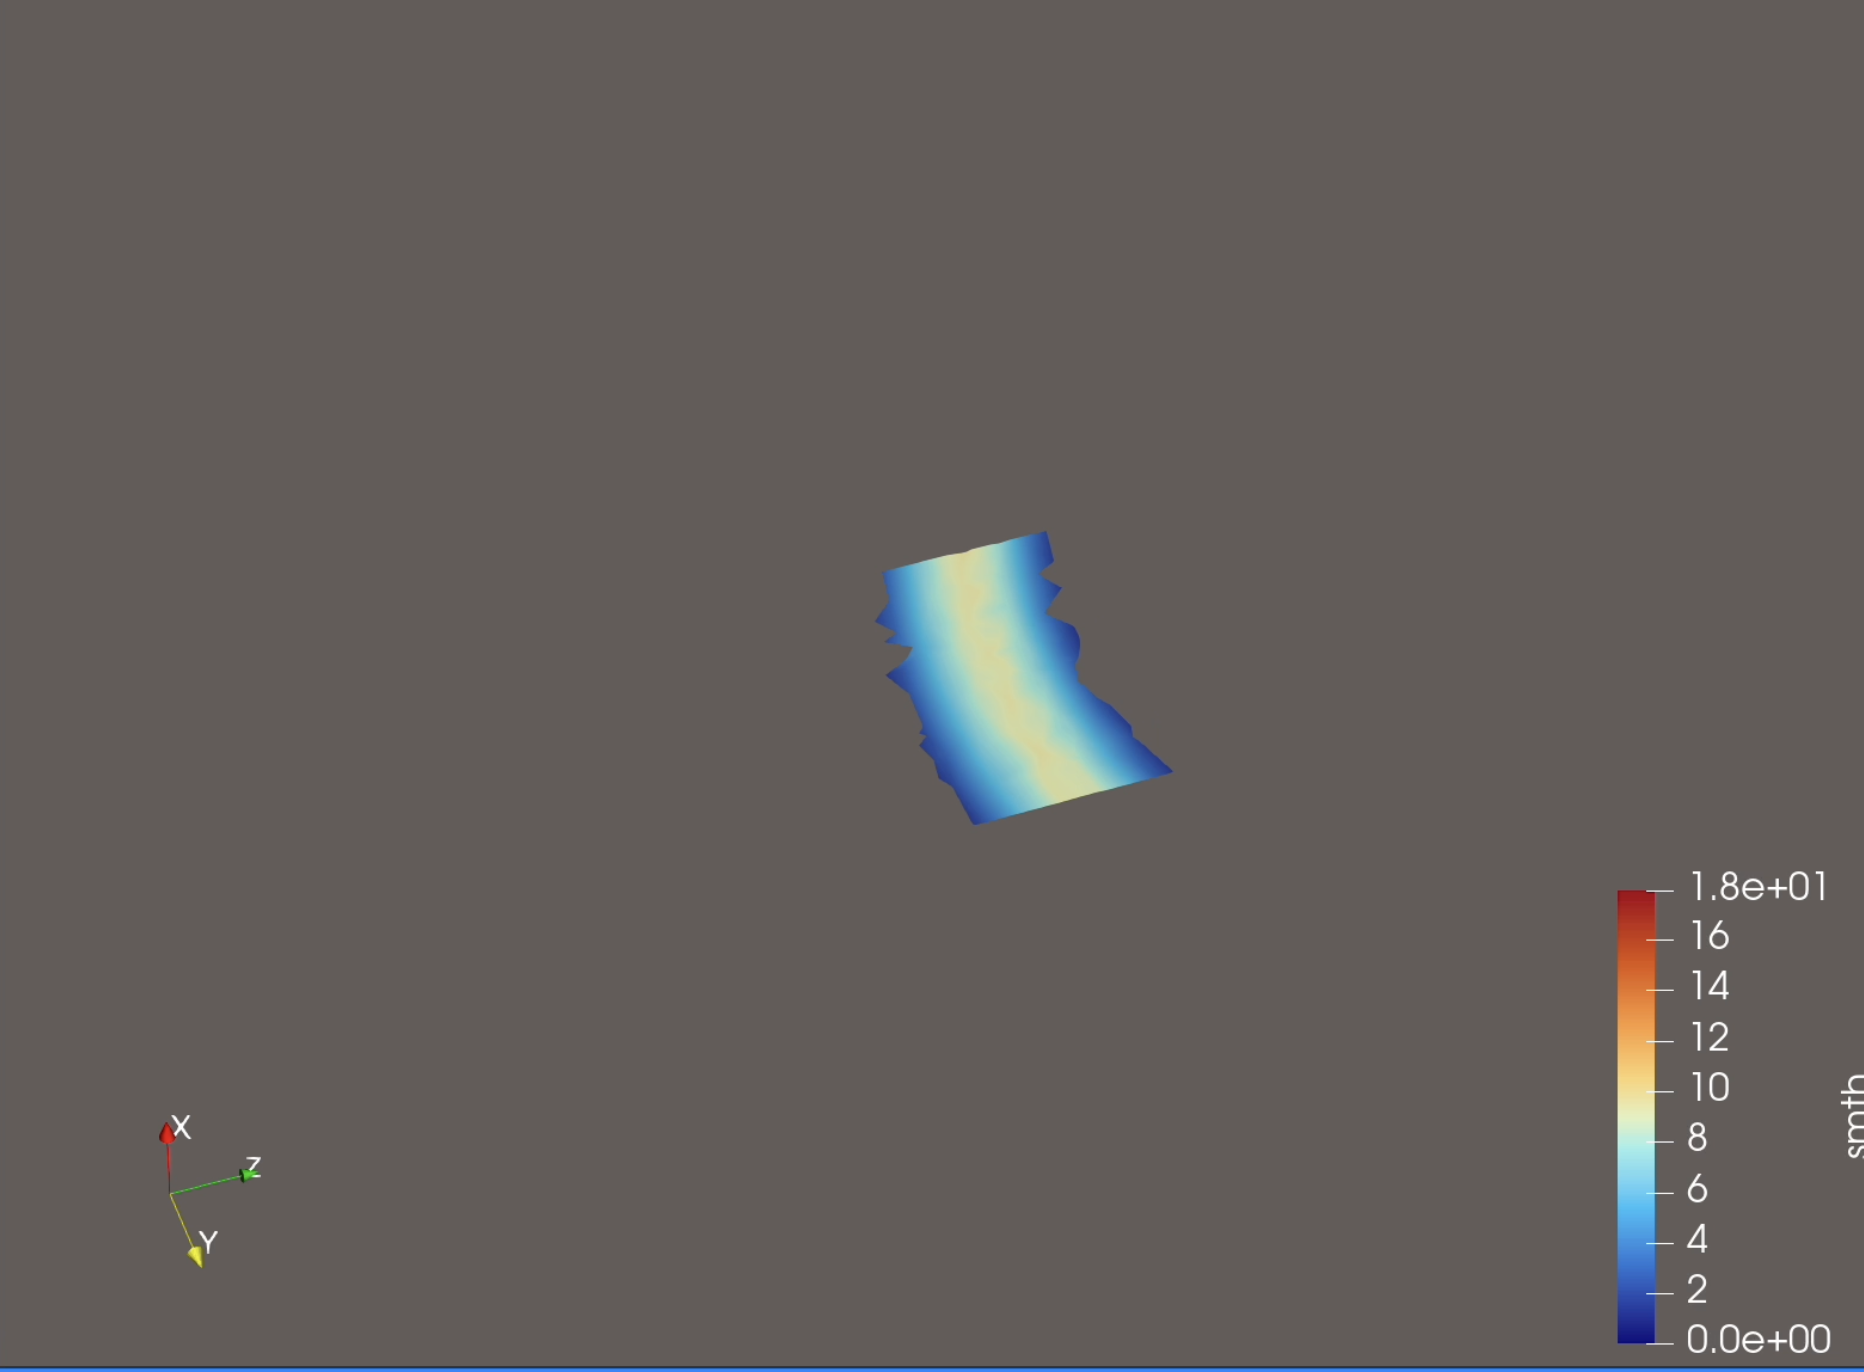
\includegraphics[width=0.8\linewidth]{img/lab2/cut.png}
  \caption{Сечение вдоль оси карандаша с полем ударной волны.}
\end{figure}

\subsection{Выводы}

Реализован цикл расчёта и визуализации нестационарного процесса:
загрузка STL-сетки через gmsh, аналитический расчёт поля волны с учётом
отражений, запись серии \texttt{.vtu}-кадров и визуализация в ParaView.
Использование неструктурированной сетки позволило корректно передать
геометрию объекта произвольной формы.
